\chapter{Chosen Ciphertext Security}\label{6-Chosen-Ciphertext-Secu}

\section{Short recap}\label{6-Short-recap}

Let's start by reviewing what we have learned so far:

\begin{itemize}
\item
  We can mathematically define security for encryption schemes. A
  natural definition is \emph{perfect secrecy}: no matter what Eve does,
  she can't learn anything about the plaintext that she didn't know
  before. Unfortunately this requires the key to be as long as the
  message, thus placing a severe limitation on the usability of it.
\item
  To get around this, we need to consider computational considerations.
  A basic object is a \emph{pseudorandom generator} and we considered
  the \emph{PRG Conjecture} which stipulates the existence of an
  efficiently computable function
  \(G:\{0,1\}^n\rightarrow\{0,1\}^{n+1}\) such that
  \(G(U_n)\approx U_{n+1}\) (where \(U_m\) denotes the uniform
  distribution on \(\{0,1\}^m\) and \(\approx\) denotes computational
  indistinguishability).
\item
  We showed that the PRG conjecture implies a pseudorandom generator of
  any polynomial output length which in particular via the stream cipher
  construction implies a computationally secure encryption with
  plaintext arbitrarily larger than the key. (The only restriction is
  that the plaintext is of polynomial size which is needed anyway if we
  want to actually be able to read and write it.)
\item
  We then showed that the PRG conjecture actually implies a stronger
  object known as a \emph{pseudorandom function (PRF) function
  collection}: this is a collection \(\{ f_s \}\) of functions such that
  if we choose \(s\) at random and fix it, and give an adversary a black
  box computing \(i \mapsto f_s(i)\) then she can't tell the difference
  between this and a blackbox computing a random function.
\item
  Pseudorandom functions turn out to be useful for \emph{identification
  protocols}, \emph{message authentication codes} and this strong notion
  of security of encryption known as \emph{chosen plaintext attack (CPA)
  security} where we are allowed to encrypt \emph{many messages of Eve's
  choice} and still require that the next message hides all information
  except for what Eve already knew before.
\end{itemize}

\section{Going beyond CPA}\label{6-Going-beyond-CPA}

It may seem that we have finally nailed down the security definition for
encryption. After all, what could be stronger than allowing Eve
unfettered access to the encryption function? Clearly an encryption
satisfying this property will hide the contents of the message in all
practical circumstances. Or will it?

\begin{pause} \label[pause]{6-Please-stop-and-play-a}

Please stop and play an ominous sound track at this point.

\end{pause}

\subsection{Example: The Wired Equivalence Protocol
(WEP)}\label{6-Example-The-Wired-Equi}

The WEP is perhaps one of the most inaccurately named protocols of all
times. It was invented in 1999 for the purpose of securing Wi-Fi
networks so that they would have virtually the same level of security as
wired networks, but already early on several security flaws were pointed
out. In particular in 2001, Fluhrer, Mantin, and Shamir showed how the
RC4 flaws we mentioned in prior lecture can be used to completely break
WEP in less than one minute. Yet, the protocol lingered on and for many
years after was still the most widely used WiFi encryption protocol as
many routers had it as the default option. In 2007 the WEP was blamed
for a hack stealing 45 million credit card numbers from T.J. Maxx. In
2012 (after 11 years of attacks!) it was estimated that it is still used
in about a quarter of encrypted wireless networks, and in 2014 it was
still the default option on many Verizon home routers. (I don't know of
more recent surveys.) Here we will talk about a different flaw of WEP
that is in fact shared by many other protocols, including the first
versions of the secure socket layer (SSL) protocol that is used to
protect all encrypted web traffic.

To avoid superfluous details we will consider a highly abstract (and
somewhat inaccurate) version of WEP that still demonstrates our main
point. In this protocol Alice (the user) sends to Bob (the access point)
an IP packet that she wants routed somewhere on the internet.

Thus we can think of the message Alice sends to Bob as a string
\(m\in\{0,1\}^\ell\) of the form \(m=(m_1,m_2)\) where \(m_1\) is the IP
address this packet needs to be routed to and \(m_2\) is the actual
message that needs to be delivered. In the WEP protocol, the message
that Alice sends to Bob has the form\\
\(E_k(m\|\ensuremath{\mathit{CRC}}(m))\) (where \(\|\) denotes
concatenation and \(\ensuremath{\mathit{CRC}}(m)\) is some cyclic
redundancy code). The actual encryption WEP used was RC4, but for us it
doesn't really matter. What does matter is that the encryption has the
form \(E_k(m') = pad \oplus m'\) where \(pad\) is computed as some
function of the key. In particular the attack we will describe works
even if we use our stronger CPA secure PRF-based scheme where
\(pad=f_k(r)\) for some random (or counter) \(r\) that is sent out
separately.

Now the security of the encryption means that an adversary seeing the
ciphertext \(c=E_k(m\|crc(m))\) will not be able to know \(m\), but
since this is traveling over the air, the adversary could ``spoof'' the
signal and send a different ciphertext \(c'\) to Bob. In particular, if
the adversary knows the IP address \(m_1\) that Alice was using (e.g.,
for example, the adversary can guess that Alice is probably one of the
billions of people that visit the website boazbarak.org on a regular
basis) then she can XOR the ciphertext with a string of her choosing and
hence convert the ciphertext
\(c = pad \oplus (m_1,m_2,\ensuremath{\mathit{CRC}}(m_1,m_2))\) into the
ciphertext \(c' = c \oplus x\) where \(x=(x_1,x_2,x_3)\) is computed so
that \(x_1 \oplus m_1\) is equal to the adversary's own IP address!

So, the adversary doesn't need to decrypt the message- by spoofing the
ciphertext she can ensure that Bob (who is an access point, and whose
job is to decrypt and then deliver packets) simply delivers it
unencrypted straight into her hands. One issue is that Eve modifies
\(m_1\) then it is unlikely that the CRC code will still check out, and
hence Bob would reject the packet. However,
\href{https://goo.gl/5aqEHB}{CRC 32} - the CRC algorithm used by WEP -
is \emph{linear} modulo \(2\), which means that for every pair of
strings \(x_1,x_2\),
\(\ensuremath{\mathit{CRC}}(m_1\oplus x_1,m_2 \oplus m_2)=\ensuremath{\mathit{CRC}}(m_1,m_2)\oplus \ensuremath{\mathit{CRC}}(x_1,x_2)\).
This means that if the original ciphertext \(c\) was an encryption of
the message \(m=(m_1,m_2,\ensuremath{\mathit{CRC}}(m_1,m_2))\) then
\(c'=c \oplus (x_1,0,\ensuremath{\mathit{CRC}}(x_1,0))\) will be an
encryption of the message
\(m'=(m_1 \oplus x_1, m_2, \ensuremath{\mathit{CRC}}(x_1\oplus m_1,m_2))\)
(where \(0\) denotes a string of zeroes of the same length as \(m_2\),
and hence \(m_2 \oplus 0 = m_2\)). Therefore by XOR'ing \(c\) with
\((x_1,0,\ensuremath{\mathit{CRC}}(x_1,0))\), the adversary Mallory can
ensure that Bob will deliver the message \(m_2\) to the IP address
\(m_1 \oplus x_1\) of her choice (see \cref{WEPattackfig}).

\begin{figure}
\centering
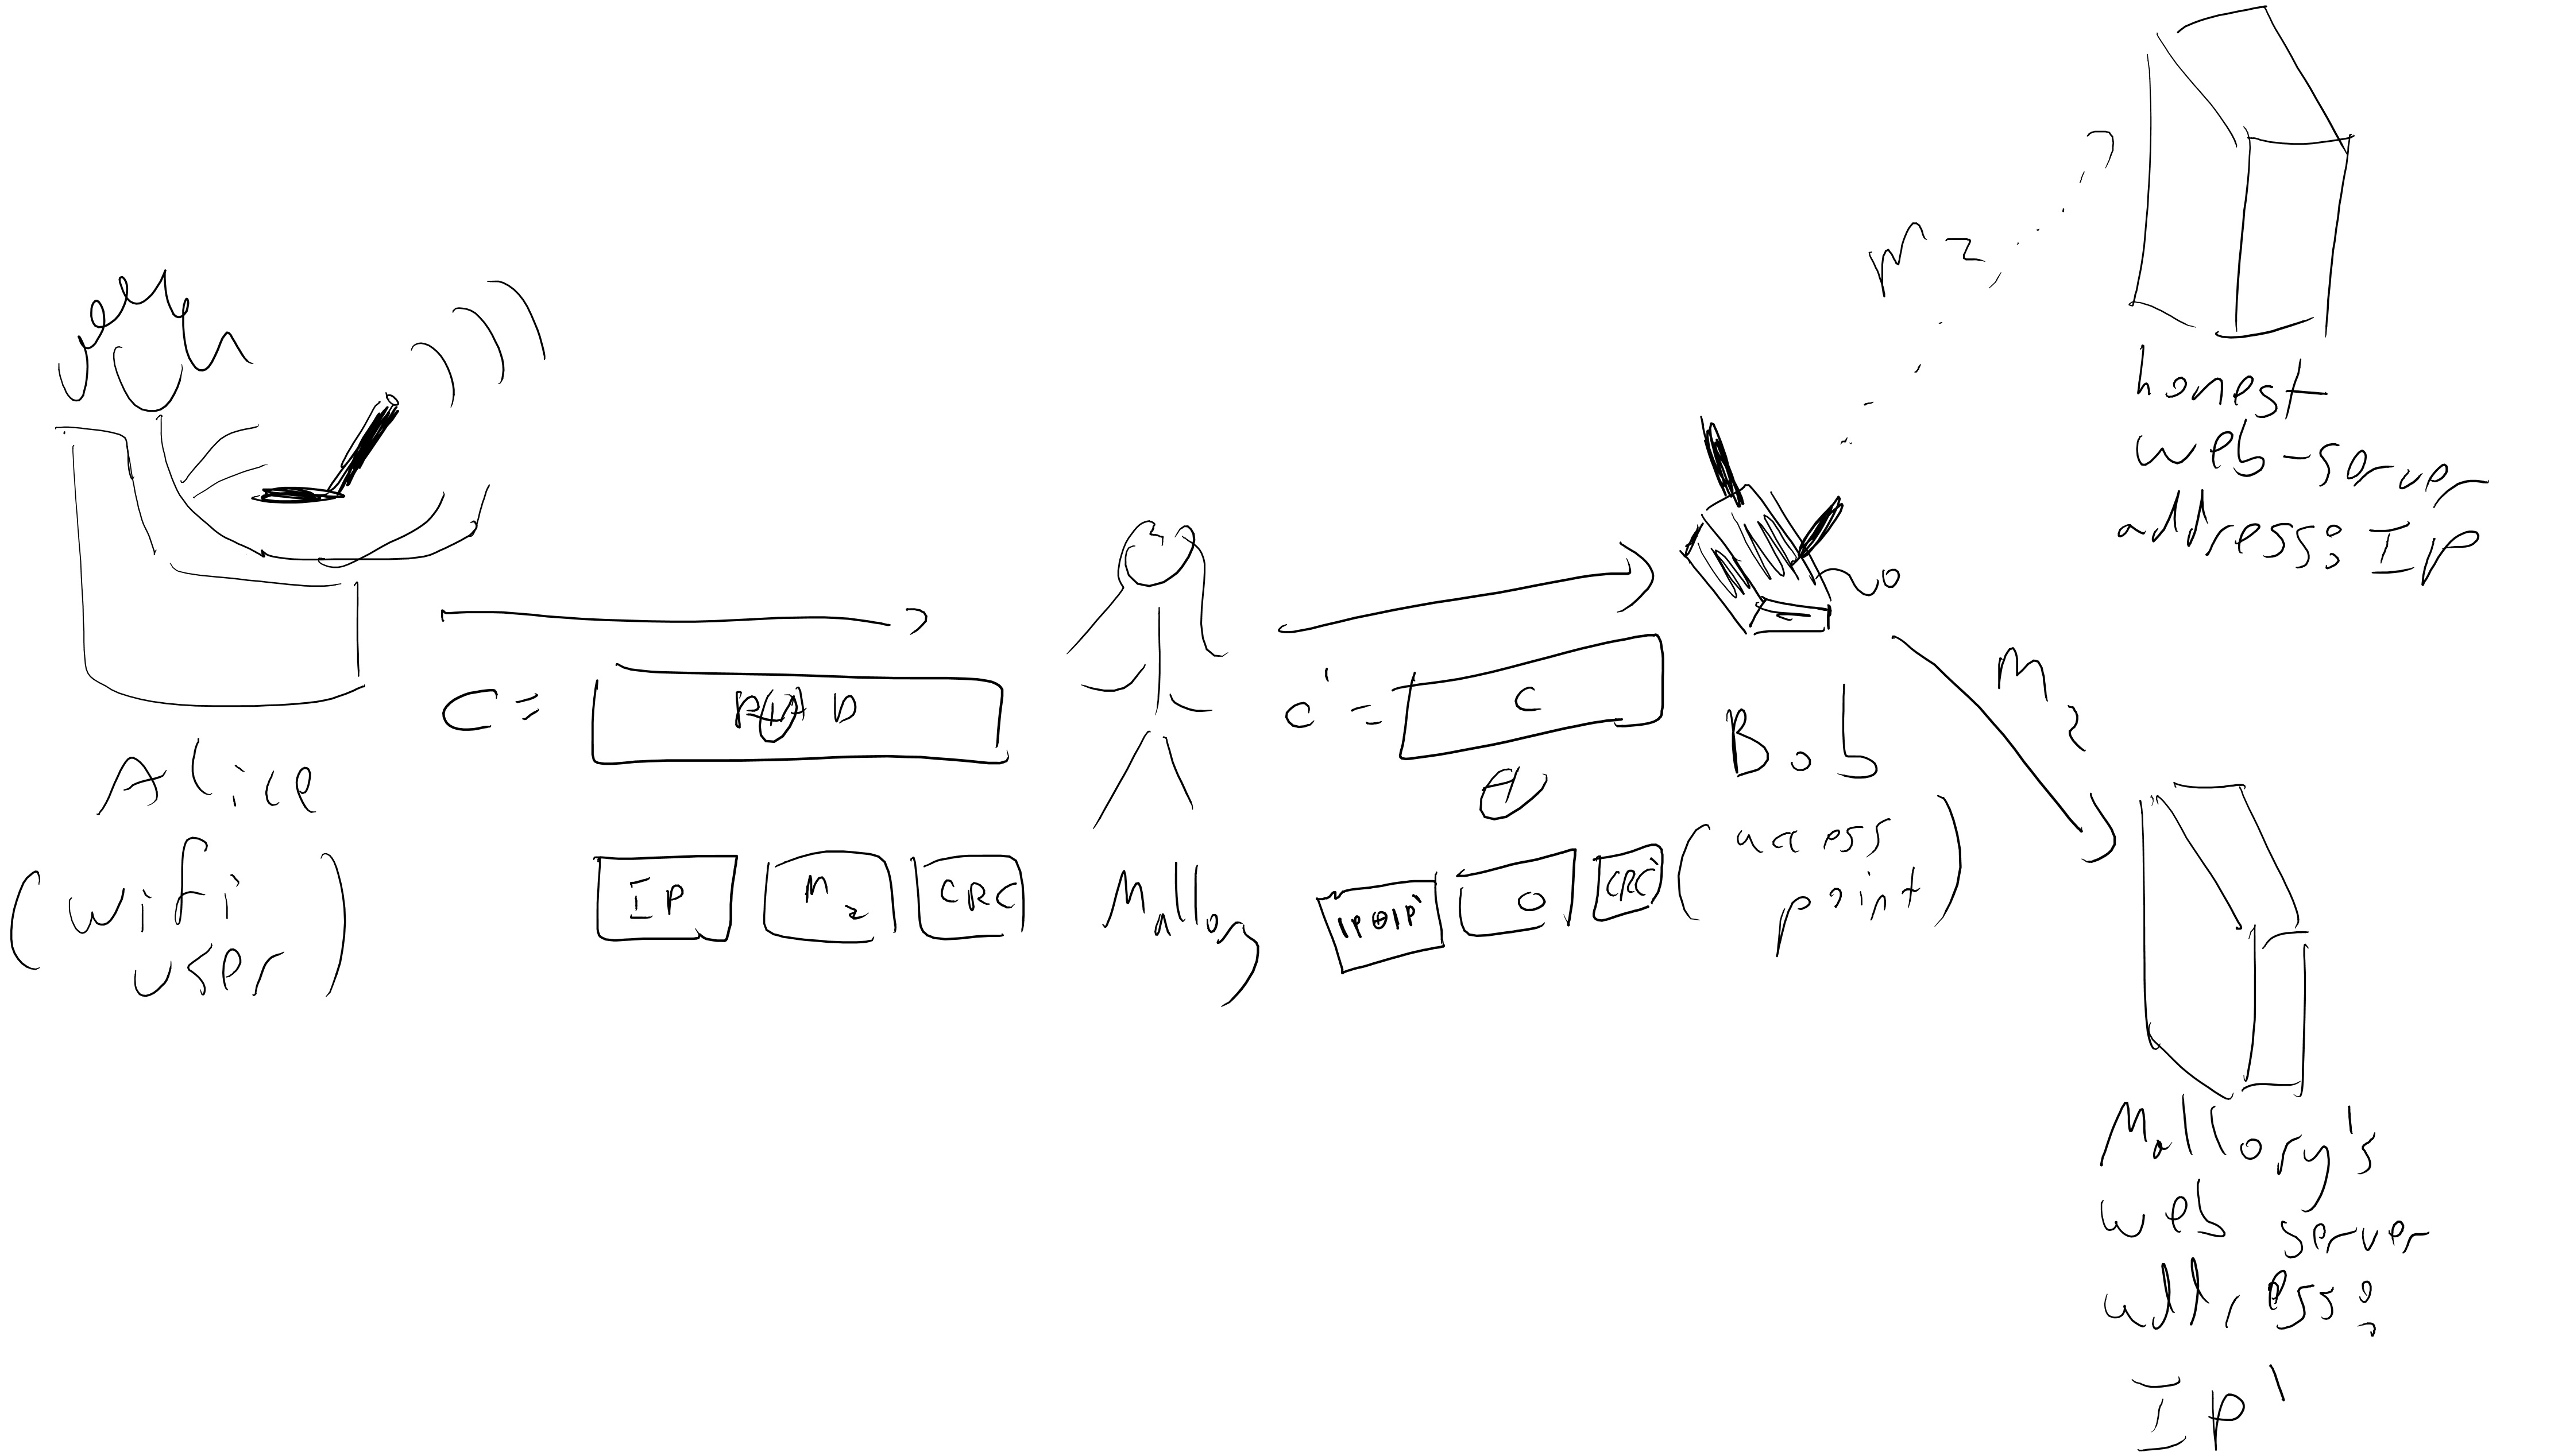
\includegraphics[width=\textwidth, height=0.25\paperheight, keepaspectratio]{../figure/wep-attack.jpg}
\caption{The attack on the WEP protocol allowing the adversary Mallory
to read encrypted messages even when Alice uses a CPA secure
encryption.}
\label{WEPattackfig}
\end{figure}

\subsection{Chosen ciphertext security}\label{6-Chosen-ciphertext-secu}

This is not an isolated example but in fact an instance of a general
pattern of many breaks in practical protocols. Some examples of
protocols broken through similar means include
\href{http://www.nds.rub.de/media/nds/veroeffentlichungen/2011/10/22/HowToBreakXMLenc.pdf}{XML
encryption},
\href{https://www.cs.columbia.edu/~smb/papers/badesp.pdf}{IPSec} (see
also \href{https://eprint.iacr.org/2005/416}{here}) as well as
JavaServer Faces, Ruby on Rails, ASP.NET, and the Steam gaming client
(see the Wikipedia page on \href{https://goo.gl/b5aKYg}{Padding Oracle
Attacks}).

The point is that often our adversaries can be \emph{active} and modify
the communication between sender and receiver, which in effect gives
them access not just to choose \emph{plaintexts} of their choice to
encrypt but even to have some impact on the \emph{ciphertexts} that are
decrypted. This motivates the following notion of security (see also
\cref{CCAgamefig}):

\hypertarget{CCAdef}{}
\begin{definition}[CCA security] \label[definition]{CCAdef}

An encryption scheme \((E,D)\) is \emph{chosen ciphertext attack (CCA)
secure} if every efficient adversary \emph{Mallory} wins in the
following game with probability at most \(1/2+ negl(n)\):\\
* Mallory gets \(1^n\) where \(n\) is the length of the key\\
* For \(poly(n)\) rounds, Mallory gets access to the functions
\(m \mapsto E_k(m)\) and \(c \mapsto D_k(c)\).\\
* Mallory chooses a pair of messages \(\{ m_0,m_1 \}\), a secret \(b\)
is chosen at random in \(\{0,1\}\), and Mallory gets
\(c^* = E_k(m_b)\).\\
* Mallory now gets another \(poly(n)\) rounds of access to the functions
\(m \mapsto E_k(m)\) and \(c \mapsto D_k(c)\) except that she is not
allowed to query \(c^*\) to her second oracle.\\
* Mallory outputs \(b'\) and \emph{wins} if \(b'=b\).

\end{definition}

\begin{marginfigure}
\centering
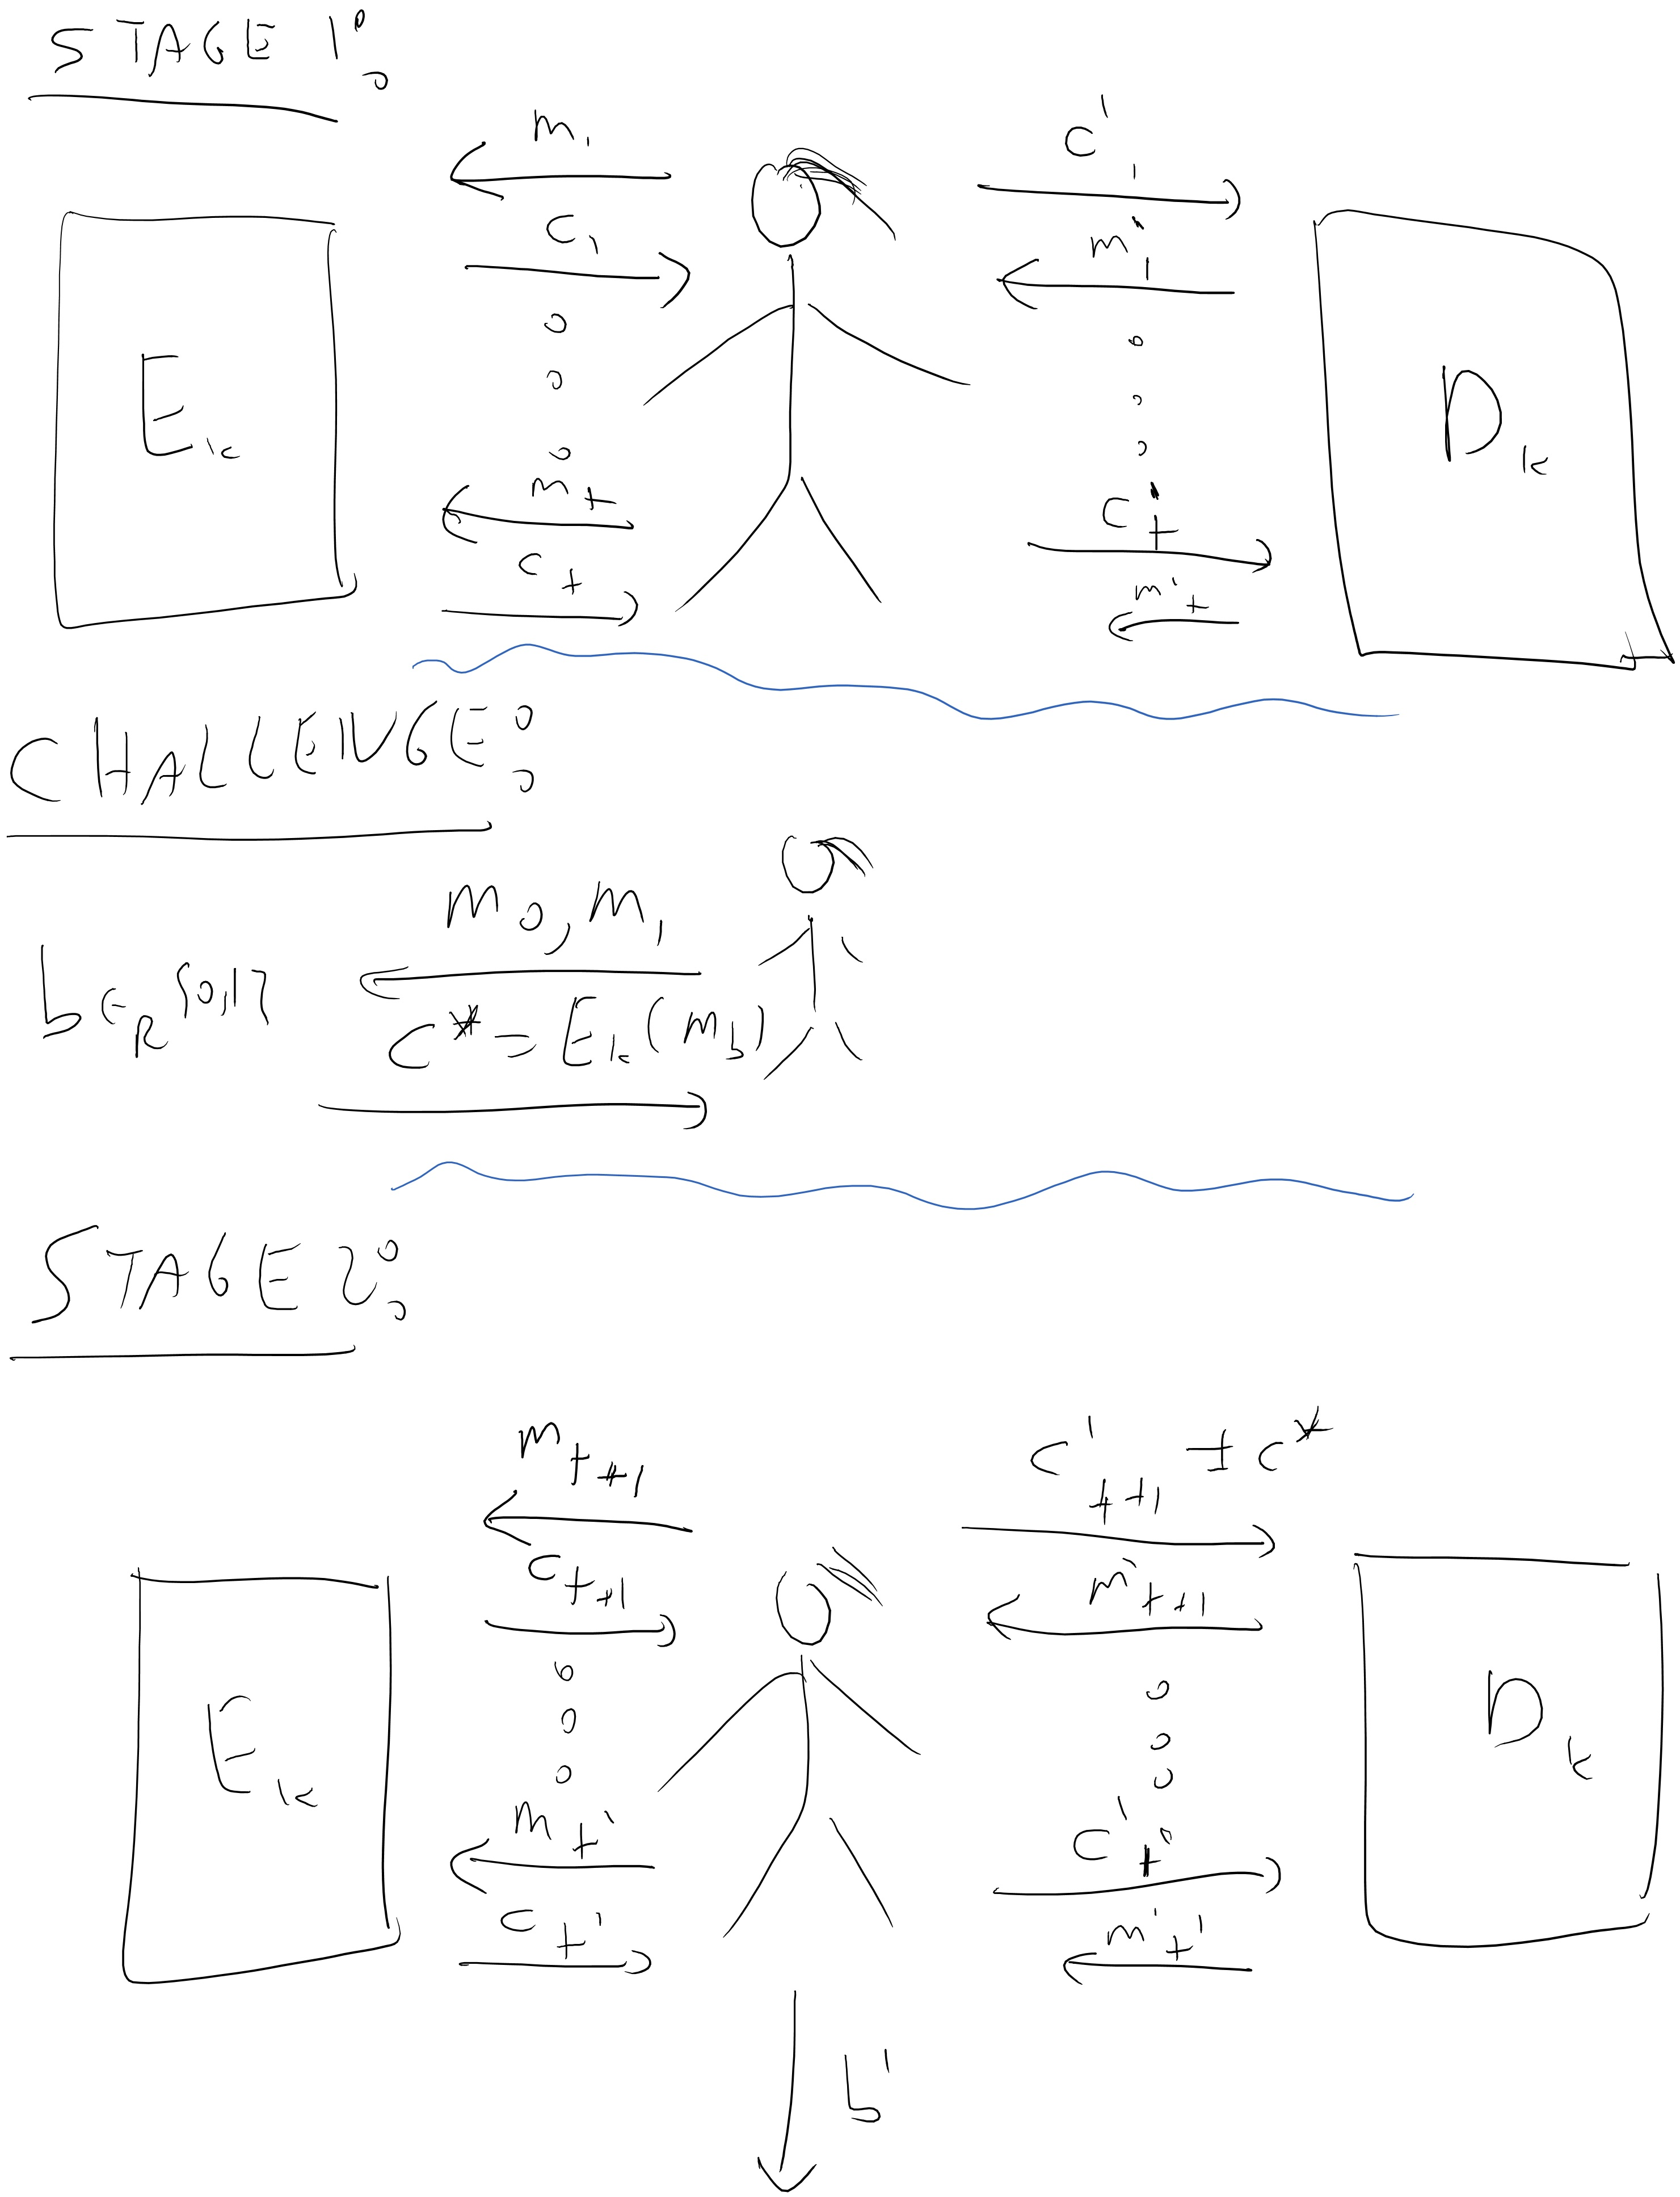
\includegraphics[width=\linewidth, height=1.5in, keepaspectratio]{../figure/cca-game.jpg}
\caption{The CCA security game.}
\label{CCAgamefig}
\end{marginfigure}

This might seems a rather strange definition so let's try to digest it
slowly. Most people, once they understand what the definition says,
don't like it that much. There are two natural objections to it:

\begin{itemize}
\tightlist
\item
  \textbf{This definition seems to be too strong:} There is no way we
  would let Mallory play with a \emph{decryption box} - that basically
  amounts to letting her break the encryption scheme. Sure, she could
  have some impact on the ciphertexts that Bob decrypts and observe some
  resulting side effects, but there is a long way from that to giving
  her oracle access to the decryption algorithm.
\end{itemize}

The response to this is that it is very hard to model what is the
``realistic'' information Mallory might get about the ciphertexts she
might cause Bob to decrypt. The goal of a security definition is not to
capture exactly the attack scenarios that occur in real life but rather
to be \emph{sufficiently conservative} so that these real life attacks
could be modeled in our game. Therefore, having a too strong definition
is not a bad thing (as long as it can be achieved!). The WEP example
shows that the definition does capture a practical issue in security and
similar attacks on practical protocols have been shown time and again
(see for example the discussion of ``padding attacks'' in Section 3.7.2
of the Katz Lindell book.)

\begin{itemize}
\tightlist
\item
  \textbf{This definition seems to be too weak:} What justification do
  we have for not allowing Mallory to make the query \(c^*\) to the
  decryption box? After all she is an adversary so she could do whatever
  she wants. The answer is that the definition would be clearly
  impossible to achieve if Mallory could simply get the decryption of
  \(c^*\) and learn whether it was an encryption of \(m_0\) or \(m_1\).
  So this restriction is the absolutely minimal one we could make
  without causing the notion to be obviously impossible. Perhaps
  surprisingly, it turns out that once we make this minimal restriction,
  we can in fact construct CCA-secure encryptions.
\end{itemize}

\paragraph{What does CCA have to do with WEP?} The CCA security game is
somewhat strange, and it might not be immediately clear whether it has
anything to do with the attack we described on the WEP protocol.
However, it turns out that using a CCA secure encryption \emph{would}
have prevented that attack. The key is the following claim:

\hypertarget{ccaweplem}{}
\begin{lemma} \label[lemma]{ccaweplem}

Suppose that \((E,D)\) is a CCA secure encryption. Then, there is no
efficient algorithm that given an encryption \(c\) of the plaintext
\((m_1,m_2)\) outputs a ciphertext \(c'\) that decrypts to
\((m'_1,m_2)\) where \(m'_1\neq m_1\).

\end{lemma}

In particular \cref{ccaweplem} rules out the attack of transforming
\(c\) that encrypts a message starting with a some address
\(\ensuremath{\mathit{IP}}\) to a ciphertext that starts with a
different address \(\ensuremath{\mathit{IP}}'\). Let us now sketch its
proof.

\begin{proof} \label[proof]{6-Well-show-that-such-if}

We'll show that such if we had an adversary \(M'\) that violates the
conclusion of the claim, then there is an adversary \(M\) that can win
in the CCA game.

The proof is simple and relies on the crucial fact that the CCA game
allows \(M\) to query the decryption box on \emph{any} ciphertext of her
choice, as long as it's not \emph{exactly identical} to the challenge
cipertext \(c^*\). In particular, if \(M'\) is able to morph an
encryption \(c\) of \(m\) to some encryption \(c'\) of some different
\(m'\) that agrees with \(m\) on some set of bits, then \(M\) can do the
following: in the security game, use \(m_0\) to be some random message
and \(m_1\) to be this plaintext \(m\). Then, when receiving \(c^*\),
apply \(M'\) to it to obtain a ciphertext \(c'\) (note that if the
plaintext differs then the ciphertext must differ also; can you see
why?) ask the decryption box to decrypt it and output \(1\) if the
resulting message agrees with \(m\) in the corresponding set of bits
(otherwise output a random bit). If \(M'\) was successful with
probability \(\epsilon\), then \(M\) would win in the CCA game with
probability at least \(1/2 + \epsilon/10\) or so.

\end{proof}

\begin{pause} \label[pause]{6-The-proof-above-is-rat}

The proof above is rather sketchy. However it is not very difficult and
proving \cref{ccaweplem} on your own is an excellent way to ensure
familiarity with the definition of CCA security.

\end{pause}

\section{Constructing CCA secure
encryption}\label{6-Constructing-CCA-secur}

The definition of CCA seems extremely strong, so perhaps it is not
surprising that it is useful, but can we actually construct it? The WEP
attack shows that the CPA secure encryption we saw before (i.e.,
\(E_k(m)=(r,f_k(r)\oplus m)\)) is \emph{not} CCA secure. We will see
other examples of \emph{non} CCA secure encryptions in the exercises.
So, how \emph{do} we construct such a scheme? The WEP attack actually
already hints of the crux of CCA security. We want to ensure that
Mallory is not able to modify the challenge ciphertext \(c^*\) to some
related \(c'\). Another way to say it is that we need to ensure the
\emph{integrity} of messages to achieve their \emph{confidentiality} if
we want to handle \emph{active} adversaries that might modify messages
on the channel. Since in in a great many practical scenarios, an
adversary might be able to do so, this is an important message that
deserves to be repeated:

\begin{quote}
\emph{To ensure confidentiality, you need integrity.}
\end{quote}

This is a lesson that has been time and again been shown and many
protocols have been broken due to the mistaken belief that if we only
care about \emph{secrecy}, it is enough to use only \emph{encryption}
(and one that is only CPA secure) and there is no need for
\emph{authentication}.
\href{http://blog.cryptographyengineering.com/2012/05/how-to-choose-authenticated-encryption.html}{Matthew
Green} writes this more provocatively as

\begin{quote}
\emph{Nearly all of the symmetric encryption modes you learned about in
school, textbooks, and Wikipedia are (potentially) insecure.\footnote{I
  also like the part where Green says about a block cipher mode that
  ``if OCB was your kid, he'd play three sports and be on his way to
  Harvard.'' We will have an exercise about a simplified version of the
  GCM mode (which perhaps only plays a single sport and is on its way to
  \ldots). You can read about OCB in Exercise 9.14 in the Boneh-Shoup
  book; it uses the notion of a ``tweakable block cipher'' which simply
  means that given a single key \(k\), you actually get a set
  \(\{ p_{k,1},\ldots,p_{k,t} \}\) of permutations that are
  indistinguishable from \(t\) independent random permutation (the set
  \(\{1,\ldots, t\}\) is called the set of ``tweaks'' and we sometimes
  index it using strings instead of numbers).}}
\end{quote}

exactly because these basic modes only ensure security for
\emph{passive} eavesdropping adversaries and do not ensure chosen
ciphertext security which is the ``gold standard'' for online
applications. (For symmetric encryption people often use the name
``authenticated encryption'' in practice rather than CCA security; those
are not identical but are extremely related notions.)

All of this suggests that Message Authentication Codes might help us get
CCA security. This turns out to be the case. But one needs to take some
care exactly \emph{how} to use MAC's to get CCA security. At this point,
you might want to stop and think how you would do this\ldots{}

\begin{pause} \label[pause]{6-You-should-stop-here-a}

You should stop here and try to think how you would implement a CCA
secure encryption by combining MAC's with a CPA secure encryption.

\end{pause}

\newpage

\begin{pause} \label[pause]{6-If-you-didnt-stop-befo}

If you didn't stop before, then you should really stop and think now.

\end{pause}

\newpage

OK, so now that you had a chance to think about this on your own, we
will describe one way that works to achieve CCA security from MACs. We
will explore other approaches that may or may not work in the exercises.

\hypertarget{CCAfromCPAMACthm}{}
\begin{theorem}[CCA from CPA and MAC] \label[theorem]{CCAfromCPAMACthm}

Let \((E,D)\) be CPA-secure encryption scheme and \((S,V)\) be a
CMA-secure MAC with \(n\) bit keys and a canonical verification
algorithm.\footnote{By a \emph{canonical verification algorithm} we mean
  that \(V_k(m,\sigma)=1\) iff \(S_k(m)=\sigma\).} Then the following
encryption \((E',D')\) with keys \(2n\) bits is CCA secure:\\
* \(E'_{k_1,k_2}(m)\) is obtained by computing \(c=E_{k_1}(m)\) ,
\(\sigma = S_{k_2}(c)\) and outputting \((c,\sigma)\).\\
* \(D'_{k_1,k_2}(c,\sigma)\) outputs nothing (e.g., an error message) if
\(V_{k_2}(c,\sigma)\neq 1\), and otherwise outputs \(D_{k_1}(c)\).

\end{theorem}

\begin{proof} \label[proof]{6-Suppose-for-the-sake-o}

Suppose, for the sake of contradiction, that there exists an adversary
\(M'\) that wins the CCA game for the scheme \((E',D')\) with
probability at least \(1/2+\epsilon\). We consider the following two
cases:

\textbf{Case I:} With probability at least \(\epsilon/10\), at some
point during the CCA game, \(M'\) sends to its decryption box a
ciphertext \((c,\sigma)\) that is not identical to one of the
ciphertexts it previously obtained from its encryption box, and obtains
from it a non-error response.

\textbf{Case II:} The event above happens with probability smaller than
\(\epsilon/10\).

We will derive a contradiction in either case. In the first case, we
will use \(M'\) to obtain an adversary that breaks the MAC \((S,V)\),
while in the second case, we will use \(M'\) to obtain an adversary that
breaks the CPA-security of \((E,D)\).

Let's start with Case I: When this case holds, we will build an
adversary \(F\) (for ``forger'') for the MAC \((S,V)\), we can assume
the adversary \(F\) has access to the both signing and verification
algorithms as black boxes for some unknown key \(k_2\) that is chosen at
random and fixed.\footnote{Since we use a MAC with canonical
  verification, access to the signature algorithm implies access to the
  verification algorithm.} \(F\) will choose \(k_1\) on its own, and
will also choose at random a number \(i_0\) from \(1\) to \(T\), where
\(T\) is the total number of queries that \(M'\) makes to the decryption
box. \(F\) will run the entire CCA game with \(M'\), using \(k_1\) and
its access to the black boxes to execute the decryption and decryption
boxes, all the way until just before \(M'\) makes the \(i_0^{th}\) query
\((c,\sigma)\) to its decryption box. At that point, \(F\) will output
\((c,\sigma)\). We claim that with probability at least
\(\epsilon/(10T)\), our forger will succeed in the CMA game in the sense
that \textbf{(i)} the query \((c,\sigma)\) will pass verification, and
\textbf{(ii)} the message \(c\) was not previously queried before to the
signing oracle.

Indeed, because we are in Case I, with probability \(\epsilon/10\), in
this game \emph{some} query that \(M'\) makes will be one that was not
asked before and hence was \emph{not} queried by \(F\) to its signing
oracle, and moreover, the returned message is not an error message, and
hence the signature passes verification. Since \(i_0\) is random, with
probability \(\epsilon/(10T)\) this query will be at the \(i_0^{th}\)
round. Let us assume that this above event
\(\ensuremath{\mathit{GOOD}}\) happened in which the \(i_0\)-th query to
the decryption box is a pair \((c,\sigma)\) that both passes
verification and the pair \((c,\sigma)\) was not returned before by the
encryption oracle. Since we pass (canonical) verification, we know that
\(\sigma=S_{k_2}(c)\), and because all encryption queries return pairs
of the form \((c',S_{k_2}(\sigma'))\), this means that no such query
returned \(c\) as its first element either. In other words, when the
event \(\ensuremath{\mathit{GOOD}}\) happens the \(i_0\)-the query
contains a pair \((c,\sigma)\) such that \(c\) was not queried before to
the signature box, but \((c,\sigma)\) passes verification. This is the
definition of breaking \((S,V)\) in a chosen message attack, and hence
we obtain a contradiction to the CMA security of \((S,V)\).

Now for Case II: In this case, we will build an adversary \(Eve\) for
CPA-game in the original scheme \((E,D)\). As you might expect, the
adversary \(Eve\) will choose by herself the key \(k_2\) for the MAC
scheme, and attempt to play the CCA security game with \(M'\). When
\(M'\) makes \emph{encryption queries} this should not be a problem-
\(Eve\) can forward the plaintext \(m\) to its encryption oracle to get
\(c=E_{k_1}(m)\) and then compute \(\sigma = S_{k_2}(c)\) since she
knows the signing key \(k_2\).

However, what does \(Eve\) do when \(M'\) makes \emph{decryption}
queries? That is, suppose that \(M'\) sends a query of the form
\((c,\sigma)\) to its decryption box. To simulate the algorithm \(D'\),
\(Eve\) will need access to a \emph{decryption box} for \(D\), but she
doesn't get such a box in the CPA game (This is a subtle point- please
pause here and reflect on it until you are sure you understand it!)

To handle this issue \(Eve\) will follow the common approach of
``winging it and hoping for the best''. When \(M'\) sends a query of the
form \((c,\sigma)\), \(Eve\) will first check if it happens to be the
case that \((c,\sigma)\) was returned before as an answer to an
encryption query \(m\). In this case \(Eve\) will breathe a sigh of
relief and simply return \(m\) to \(M'\) as the answer. (This is
obviously correct: if \((c,\sigma)\) is the encryption of \(m\) then
\(m\) is the decryption of \((c,\sigma)\).) However, if the query
\((c,\sigma)\) has not been returned before as an answer, then \(Eve\)
is in a bit of a pickle. The way out of it is for her to simply return
``error'' and hope that everything will work out. The crucial
observation is that because we are in case II things \emph{will} work
out. After all, the only way \(Eve\) makes a mistake is if she returns
an error message where the original decryption box would not have done
so, but this happens with probability at most \(\epsilon/10\). Hence, if
\(M'\) has success \(1/2+\epsilon\) in the CCA game, then even if it's
the case that \(M'\) always outputs the wrong answer when \(Eve\) makes
this mistake, we will still get success at least \(1/2+0.9\epsilon\).
Since \(\epsilon\) is non negligible, this would contradict the CPA
security of \((E,D)\) thereby concluding the proof of the theorem.

\end{proof}

\begin{pause} \label[pause]{6-This-proof-is-emblemat}

This proof is emblematic of a general principle for proving CCA
security. The idea is to show that the decryption box is completely
``useless'' for the adversary, since the only way to get a non error
response from it is to feed it with a ciphertext that was received from
the encryption box.

\end{pause}

\section{(Simplified) GCM encryption}\label{6-Simplified-GCM-encrypt}

The construction above works as a generic construction, but it is
somewhat costly in the sense that we need to evaluate both the block
cipher and the MAC. In particular, if messages have \(t\) blocks, then
we would need to invoke two cryptographic operations (a block cipher
encryption and a MAC computation) per block. The
\href{https://goo.gl/uz6WgS}{GCM (Galois Counter Mode)} is a way around
this. We are going to describe a simplified version of this mode. For
simplicity, assume that the number of blocks \(t\) is fixed and known
(though many of the annoying but important details in block cipher modes
of operations involve dealing with padding to multiple of blocks and
dealing with variable block size).

A \href{https://goo.gl/jLpNtU}{universal hash function collection} is a
family of functions \(\{ h:\{0,1\}^\ell\rightarrow\{0,1\}^n \}\) such
that for every \(x \neq x' \in \{0,1\}^\ell\), the random variables
\(h(x)\) and \(h(x')\) (taken over the choice of a random \(h\) from
this family) are pairwise independent in \(\{0,1\}^{2n}\). That is, for
every two potential outputs \(y,y'\in \{0,1\}^n\), \[
\Pr_h[ h(x)=y \;\wedge\; h(x')=y']=2^{-2n} \label{equnivhash}
\]

Universal hash functions have rather efficient constructions, and in
particular if we relax the definition to allow \emph{almost universal}
hash functions (where we replace the \(2^{-2n}\) factor in the righthand
side of \eqref{equnivhash} by a slightly bigger, though still negligible
quantity) then the constructions become extremely efficient and the size
of the description of \(h\) is only related to \(n\), no matter how big
\(\ell\) is.\footnote{In \(\epsilon\)-almost universal hash functions we
  require that for every \(y,y'\in \{0,1\}^{n}\), and
  \(x\neq x' \in \{0,1\}^\ell\), the probability that \(h(x)= h(x')\) is
  at most \(\epsilon\). It can be easily shown that the analysis below
  extends to \(\epsilon\) almost universal hash functions as long as
  \(\epsilon\) is negligible, but we will leave verifying this to the
  reader.}

Our encryption scheme is defined as follow. The key is \((k,h)\) where
\(k\) is an index to a pseudorandom permutation \(\{ p_k \}\) and \(h\)
is the key for a \emph{universal hash function}.\footnote{In practice
  the key \(h\) is derived from the key \(k\) by applying the PRP to
  some particular input.} To encrypt a message
\(m = (m_1,\ldots,m_t) \in \{0,1\}^{nt}\) do the following:

\begin{itemize}
\item
  Choose \(\ensuremath{\mathit{IV}}\) at random in \([2^n]\).
\item
  Let \(z_i = E(k,\ensuremath{\mathit{IV}}+i)\) for \(i=1,\ldots,t+1\).
\item
  Let \(c_i = z_i \oplus m_i\).
\item
  Let \(c_{t+1} = h(c_1,\ldots,c_t) \oplus z_{t+1}\).
\item
  Output \((\ensuremath{\mathit{IV}},c_1,\ldots,c_{t+1})\).
\end{itemize}

The communication overhead includes one additional output block plus the
IV (whose transmission can often be avoided or reduced, depending on the
settings; see the notion of ``nonce based encryption''). This is fairly
minimal. The additional computational cost on top of \(t\) block-cipher
evaluation is the application of \(h(\cdot)\). For the particular choice
of \(h\) used in Galois Counter Mode, this function \(h\) can be
evaluated very efficiently- at a cost of a single multiplication in the
Galois field of size \(2^{128}\) per block (one can think of it as some
very particular operation that maps two \(128\) bit strings to a single
one, and can be carried out quite efficiently). We leave it as an
(excellent!) exercise to prove that the resulting scheme is CCA secure.

\section{Padding, chopping, and their pitfalls: the ``buffer overflow''
of cryptography}\label{6-Padding-chopping-and-t}

In this course we typically focus on the simplest case where messages
have a \emph{fixed size}. But in fact, in real life we often need to
chop long messages into blocks, or pad messages so that their length
becomes an integral multiple of the block size. Moreover, there are
several subtle ways to get this wrong, and these have been used in
several practical attacks.

\paragraph{Chopping into blocks:} A block cipher a-priori provides a way
to encrypt a message of length \(n\), but we often have much longer
messages and need to ``chop'' them into blocks. This is where the
\emph{block cipher modes} discussed in the previous lecture come in.
However, the basic popular modes such as CBC and OFB do \emph{not}
provide security against chosen ciphertext attack, and in fact typically
make it easy to \emph{extend} a ciphertext with an additional block or
to \emph{remove} the last block from a ciphertext, both being operations
which should not be feasible in a CCA secure encryption.

\paragraph{Padding:} Oftentimes messages are not an integer multiple of
the block size and hence need to be \emph{padded}. The \emph{padding} is
typically a map that takes the last partial block of the message (i.e.,
a string \(m\) of length in \(\{0,\ldots,n-1\}\)) and maps it into a
full block (i.e., a string \(m\in\{0,1\}^n\)). The map needs to be
invertible which in particular means that if the message is already an
integer multiple of the block size we will need to add an extra block.
(Since we have to map all the \(1+2+\ldots+2^{n-1}\) messages of length
\(1,\ldots,n-1\) into the \(2^n\) messages of length \(n\) in a
one-to-one fashion.) One approach for doing so is to pad an \(n'<n\)
length message with the string \(10^{n-n'-1}\). Sometimes people use a
different padding which involves encoding the length of the pad.

\section{Chosen ciphertext attack as implementing
metaphors}\label{6-Chosen-ciphertext-atta}

The classical ``metaphor'' for an encryption is a sealed envelope, but
as we have seen in the WEP, this metaphor can lead you astray. If you
placed a message \(m\) in a sealed envelope, you should not be able to
modify it to the message \(m \oplus m'\) without opening the envelope,
and yet this is exactly what happens in the canonical CPA secure
encryption \(E_k(m)=(r,f_k(r) \oplus m)\). CCA security comes much
closer to realizing the metaphor, and hence is considered as the ``gold
standard'' of secure encryption. This is important even if you do not
intend to write poetry about encryption. \emph{Formal verification} of
computer programs is an area that is growing in importance given that
computer programs become both more complex and more mission critical.
Cryptographic protocols can fail in subtle ways, and even published
proofs of security can turn out to have bugs in them. Hence there is a
line of research dedicated to finding ways to \emph{automatically} prove
security of cryptographic protocols. Much of these line of research is
based on simple models to describe protocols that are known as
\emph{Dolev Yao models}, based on the first paper that proposed such
models. These models define an \emph{algebraic} form of security, where
rather than thinking of messages, keys, and ciphertexts as binary
string, we think of them as abstract entities. There are certain rules
for manipulating these symbols. For example, given a key \(k\) and a
message \(m\) you can create the ciphertext \(\{ m \}_k\), which you can
decrypt back to \(m\) using the same key. However the assumption is that
any information that cannot be obtained by such manipulation is unknown.

Translating a proof of security in this algebra to a proof for real
world adversaries is highly non trivial. However, to have even a
fighting chance, the encryption scheme needs to be as strong as
possible, and in particular it turns out that security notions such as
CCA play a crucial role.
